%% Preamble for this document
% Declare the document class with 12pt font
\documentclass[11pt]{article}
% Include the math package
\usepackage{amsmath}
% Use the geometry package to change the margins to 1"
\usepackage[margin=1in]{geometry}
% Include the graphicx package for inserting diagrams of the problem
\usepackage{graphicx}

% Here's the document
\begin{document}

	% Create the title page
	\thispagestyle{empty}
	\pagenumbering{gobble}
	\title{MATH 189: Induction Proof}
	\author{Rob Peterson}
	\date{Fall 2017}
	\maketitle

	\newpage % Force a page break for the title page

	\pagenumbering{arabic} % Re-Start the page numbering

	%% Introduction section
	\section{Introduction}
		The problem under consideration in this document is a problem consisting of disks, an algorithm and a series of steps.  
		The problem is described as follows:\
		\begin{align}
			1) &\text{ A stack of seven disks sits on a surface.}\\
			2) &\text{ One disk is added to the top of the existing stack(s),} \\
		    	    &\text{ and a set of disks is added to form a square perimeter around the existing stack(s).}\\
			3) &\text{ Step 2 is repeated ad Infinium.}
		\end{align}	
		It is often easier to understand a problem if there are visual references available to the reader.  The author has provided these below:\
		\begin{figure}[h]
			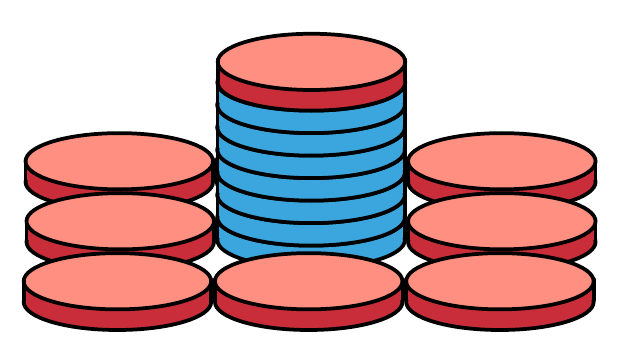
\includegraphics{step1.png}
			\caption{Step 1}
			\label{Step1_ortho}
			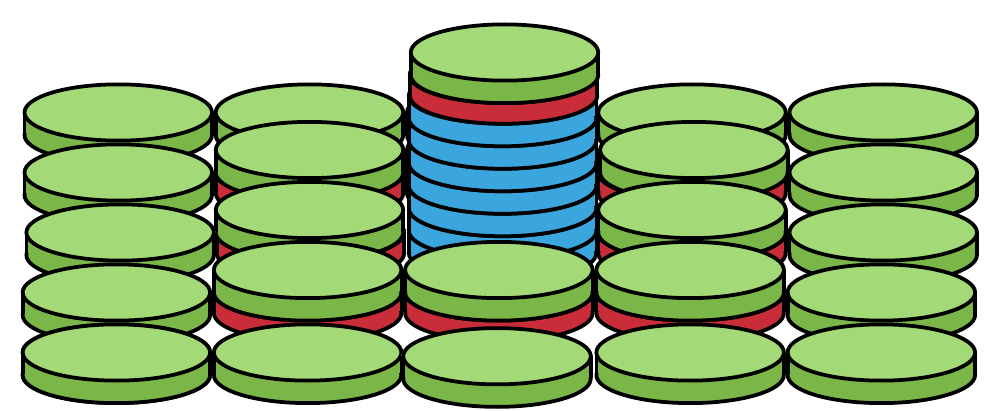
\includegraphics{step2.png}
			\caption{Step 2}
			\label{Step2_ortho}
		\end{figure}
	\newpage
	\section{Recursive and closed form expressions}
		The ultimate goal is to use the principle of mathematical induction to prove the validity of a closed form expression 
		for describing the number of disks needed for any particular step of the problem statement.  This will involve four 
		steps; generating data, developing a recursive formula, developing a closed form expression, and finally using induction 
 		prove the close form to be correct.
	
	\subsection{Data}
		

	\begin{align}
		D(n)&= D(k-1)+(2k-3)^3+2(2k-1)+2(2k-3)\\
		D(k+1)&=D(k)+(2(k+1)-3)^2+2(2(k+1)-1)+2(2(k+1)-3)\\
		&=D(k)+(2k+2-3)^2+2(2k+2-1)+2(2k+2-3)\\
		&=D(k)+(2k-1)^2+2(2k+1)+2(2k-1)\\
		&=D(k)+(2k-1)^2+4k+2+4k-2\\
		&=D(k)+4k^2-4k+1+4k+2+4k-2\\
		&=D(k)+4k^2+4k+1		
	\end{align}
	\text{We've assumed that the closed form formula is valid for D(k)}
	\begin{align}
		D(k+1)&=[\frac{4}{3}k^3-\frac{1}{3}k+6]+4k^2+4k+1\\	
		&=\frac{4k^3-k+18}{3}+4k^2+4k+1\\
		&=\frac{4k^3-k+18+12k^2+12k+3}{3}\\
		&=\frac{4k^3+12k^2+11k+21}{3}\\
		&=\frac{4k^3+12k^2+(12k-1k)+(-1+18+4)}{3}\\
		&=\frac{[4k^3+12k^2+12k+4]+[-1k-1]+18)}{3}\\
		&=\frac{4[k^3+3k^2+3k+1]-[k+1]+18)}{3}\\
		&=\frac{4(k+1)^3-(k+1)+18)}{3}\\
		&=\frac{4(k+1)^3}{3}-\frac{(k+1)}{3}+6
	\end{align}
	By mathematial induction, the preceding has proven that the closed form formula expressed in equation 12 accurately describes how many 
	disks would be needed to complete any particular step in the problem statement.
\end{document}